\documentclass[a4paper]{article}

\def\npart {III}
\def\nterm {Lent}
\def\nyear {2017}
\def\nlecturer {D. B. Skinner}
\def\ncourse {Advanced Quantum Field Theory}
\def\nlectures {MWF.11}

% Imports
\ifx \nextra \undefined
  \usepackage[pdftex,
    hidelinks,
    pdfauthor={Dexter Chua},
    pdfsubject={Cambridge Maths Notes: Part \npart\ - \ncourse},
    pdftitle={Part \npart\ - \ncourse},
  pdfkeywords={Cambridge Mathematics Maths Math \npart\ \nterm\ \nyear\ \ncourse}]{hyperref}
  \title{Part \npart\ - \ncourse}
\else
  \usepackage[pdftex,
    hidelinks,
    pdfauthor={Dexter Chua},
    pdfsubject={Cambridge Maths Notes: Part \npart\ - \ncourse\ (\nextra)},
    pdftitle={Part \npart\ - \ncourse\ (\nextra)},
  pdfkeywords={Cambridge Mathematics Maths Math \npart\ \nterm\ \nyear\ \ncourse\ \nextra}]{hyperref}

  \title{Part \npart\ - \ncourse \\ {\Large \nextra}}
\fi

\author{Lectured by \nlecturer \\\small Notes taken by Dexter Chua}
\date{\nterm\ \nyear}

\usepackage{alltt}
\usepackage{amsfonts}
\usepackage{amsmath}
\usepackage{amssymb}
\usepackage{amsthm}
\usepackage{booktabs}
\usepackage{caption}
\usepackage{enumitem}
\usepackage{fancyhdr}
\usepackage{graphicx}
\usepackage{mathtools}
\usepackage{microtype}
\usepackage{multirow}
\usepackage{pdflscape}
\usepackage{pgfplots}
\usepackage{siunitx}
\usepackage{tabularx}
\usepackage{tikz}
\usepackage{tkz-euclide}
\usepackage[normalem]{ulem}
\usepackage[all]{xy}

\pgfplotsset{compat=1.12}

\pagestyle{fancyplain}
\lhead{\emph{\nouppercase{\leftmark}}}
\ifx \nextra \undefined
  \rhead{
    \ifnum\thepage=1
    \else
      \npart\ \ncourse
    \fi}
\else
  \rhead{
    \ifnum\thepage=1
    \else
      \npart\ \ncourse\ (\nextra)
    \fi}
\fi
\usetikzlibrary{arrows}
\usetikzlibrary{decorations.markings}
\usetikzlibrary{decorations.pathmorphing}
\usetikzlibrary{positioning}
\usetikzlibrary{fadings}
\usetikzlibrary{intersections}
\usetikzlibrary{cd}

\newcommand*{\Cdot}{\raisebox{-0.25ex}{\scalebox{1.5}{$\cdot$}}}
\newcommand {\pd}[2][ ]{
  \ifx #1 { }
    \frac{\partial}{\partial #2}
  \else
    \frac{\partial^{#1}}{\partial #2^{#1}}
  \fi
}

% Theorems
\theoremstyle{definition}
\newtheorem*{aim}{Aim}
\newtheorem*{axiom}{Axiom}
\newtheorem*{claim}{Claim}
\newtheorem*{cor}{Corollary}
\newtheorem*{defi}{Definition}
\newtheorem*{eg}{Example}
\newtheorem*{fact}{Fact}
\newtheorem*{law}{Law}
\newtheorem*{lemma}{Lemma}
\newtheorem*{notation}{Notation}
\newtheorem*{prop}{Proposition}
\newtheorem*{thm}{Theorem}

\renewcommand{\labelitemi}{--}
\renewcommand{\labelitemii}{$\circ$}
\renewcommand{\labelenumi}{(\roman{*})}

\let\stdsection\section
\renewcommand\section{\newpage\stdsection}

% Strike through
\def\st{\bgroup \ULdepth=-.55ex \ULset}

% Maths symbols
\newcommand{\bra}{\langle}
\newcommand{\ket}{\rangle}

\newcommand{\N}{\mathbb{N}}
\newcommand{\Z}{\mathbb{Z}}
\newcommand{\Q}{\mathbb{Q}}
\renewcommand{\H}{\mathbb{H}}
\newcommand{\R}{\mathbb{R}}
\newcommand{\C}{\mathbb{C}}
\newcommand{\Prob}{\mathbb{P}}
\renewcommand{\P}{\mathbb{P}}
\newcommand{\E}{\mathbb{E}}
\newcommand{\F}{\mathbb{F}}
\newcommand{\cU}{\mathcal{U}}
\newcommand{\RP}{\mathbb{RP}}
\newcommand{\CP}{\mathbb{CP}}

\newcommand{\ph}{\,\cdot\,}

\DeclareMathOperator{\sech}{sech}
\DeclareMathOperator{\cosech}{cosech}
\DeclareMathOperator{\cosec}{cosec}

\DeclareMathOperator{\covol}{covol}
\DeclareMathOperator{\vol}{vol}

\let\Im\relax
\let\Re\relax
\DeclareMathOperator{\Im}{Im}
\DeclareMathOperator{\Re}{Re}
\DeclareMathOperator{\im}{im}
\DeclareMathOperator{\image}{image}
\DeclareMathOperator{\Ann}{Ann}

\DeclareMathOperator*{\res}{res}
\DeclareMathOperator{\Res}{Res}
\DeclareMathOperator{\Ind}{Ind}

\DeclareMathOperator{\tr}{tr}
\DeclareMathOperator{\diag}{diag}
\DeclareMathOperator{\rank}{rank}
\DeclareMathOperator{\card}{card}
\DeclareMathOperator{\spn}{span}
\DeclareMathOperator{\adj}{adj}

\DeclareMathOperator{\erf}{erf}
\DeclareMathOperator{\erfc}{erfc}

\DeclareMathOperator{\ord}{ord}
\DeclareMathOperator{\Sym}{Sym}

\DeclareMathOperator{\sgn}{sgn}
\DeclareMathOperator{\orb}{orb}
\DeclareMathOperator{\stab}{stab}
\DeclareMathOperator{\ccl}{ccl}

\DeclareMathOperator{\lcm}{lcm}
\DeclareMathOperator{\hcf}{hcf}

\DeclareMathOperator{\Int}{Int}
\DeclareMathOperator{\id}{id}

\DeclareMathOperator{\betaD}{beta}
\DeclareMathOperator{\gammaD}{gamma}
\DeclareMathOperator{\Poisson}{Poisson}
\DeclareMathOperator{\binomial}{binomial}
\DeclareMathOperator{\multinomial}{multinomial}
\DeclareMathOperator{\Bernoulli}{Bernoulli}
\DeclareMathOperator{\like}{like}

\DeclareMathOperator{\var}{var}
\DeclareMathOperator{\cov}{cov}
\DeclareMathOperator{\bias}{bias}
\DeclareMathOperator{\mse}{mse}
\DeclareMathOperator{\corr}{corr}

\DeclareMathOperator{\otp}{otp}
\DeclareMathOperator{\dom}{dom}

\DeclareMathOperator{\Root}{Root}
\DeclareMathOperator{\supp}{supp}
\DeclareMathOperator{\rel}{rel}
\DeclareMathOperator{\Hom}{Hom}
\DeclareMathOperator{\Aut}{Aut}
\DeclareMathOperator{\Gal}{Gal}
\DeclareMathOperator{\Mat}{Mat}
\DeclareMathOperator{\End}{End}
\DeclareMathOperator{\Char}{char}
\DeclareMathOperator{\ev}{ev}
\DeclareMathOperator{\St}{St}
\DeclareMathOperator{\Lk}{Lk}
\DeclareMathOperator{\disc}{disc}
\DeclareMathOperator{\Isom}{Isom}
\DeclareMathOperator{\length}{length}
\DeclareMathOperator{\energy}{energy}
\DeclareMathOperator{\area}{area}
\DeclareMathOperator{\Syl}{Syl}
\DeclareMathOperator{\cl}{cl}
\DeclareMathOperator{\fix}{fix}

\newcommand{\GL}{\mathrm{GL}}
\newcommand{\SL}{\mathrm{SL}}
\newcommand{\PGL}{\mathrm{PGL}}
\newcommand{\PSL}{\mathrm{PSL}}
\newcommand{\PSU}{\mathrm{PSU}}
\newcommand{\Or}{\mathrm{O}}
\newcommand{\SO}{\mathrm{SO}}
\newcommand{\U}{\mathrm{U}}
\newcommand{\SU}{\mathrm{SU}}

\renewcommand{\d}{\mathrm{d}}
\newcommand{\D}{\mathrm{D}}

\tikzset{->/.style = {decoration={markings,
                                  mark=at position 1 with {\arrow[scale=2]{latex'}}},
                      postaction={decorate}}}
\tikzset{<-/.style = {decoration={markings,
                                  mark=at position 0 with {\arrowreversed[scale=2]{latex'}}},
                      postaction={decorate}}}
\tikzset{<->/.style = {decoration={markings,
                                   mark=at position 0 with {\arrowreversed[scale=2]{latex'}},
                                   mark=at position 1 with {\arrow[scale=2]{latex'}}},
                       postaction={decorate}}}
\tikzset{->-/.style = {decoration={markings,
                                   mark=at position #1 with {\arrow[scale=2]{latex'}}},
                       postaction={decorate}}}
\tikzset{-<-/.style = {decoration={markings,
                                   mark=at position #1 with {\arrowreversed[scale=2]{latex'}}},
                       postaction={decorate}}}

\tikzset{circ/.style = {fill, circle, inner sep = 0, minimum size = 3}}
\tikzset{mstate/.style={circle, draw, blue, text=black, minimum width=0.7cm}}

\definecolor{mblue}{rgb}{0.2, 0.3, 0.8}
\definecolor{morange}{rgb}{1, 0.5, 0}
\definecolor{mgreen}{rgb}{0.1, 0.4, 0.2}
\definecolor{mred}{rgb}{0.5, 0, 0}

\def\drawcirculararc(#1,#2)(#3,#4)(#5,#6){%
    \pgfmathsetmacro\cA{(#1*#1+#2*#2-#3*#3-#4*#4)/2}%
    \pgfmathsetmacro\cB{(#1*#1+#2*#2-#5*#5-#6*#6)/2}%
    \pgfmathsetmacro\cy{(\cB*(#1-#3)-\cA*(#1-#5))/%
                        ((#2-#6)*(#1-#3)-(#2-#4)*(#1-#5))}%
    \pgfmathsetmacro\cx{(\cA-\cy*(#2-#4))/(#1-#3)}%
    \pgfmathsetmacro\cr{sqrt((#1-\cx)*(#1-\cx)+(#2-\cy)*(#2-\cy))}%
    \pgfmathsetmacro\cA{atan2(#2-\cy,#1-\cx)}%
    \pgfmathsetmacro\cB{atan2(#6-\cy,#5-\cx)}%
    \pgfmathparse{\cB<\cA}%
    \ifnum\pgfmathresult=1
        \pgfmathsetmacro\cB{\cB+360}%
    \fi
    \draw (#1,#2) arc (\cA:\cB:\cr);%
}
\newcommand\getCoord[3]{\newdimen{#1}\newdimen{#2}\pgfextractx{#1}{\pgfpointanchor{#3}{center}}\pgfextracty{#2}{\pgfpointanchor{#3}{center}}}

\def\Xint#1{\mathchoice
   {\XXint\displaystyle\textstyle{#1}}%
   {\XXint\textstyle\scriptstyle{#1}}%
   {\XXint\scriptstyle\scriptscriptstyle{#1}}%
   {\XXint\scriptscriptstyle\scriptscriptstyle{#1}}%
   \!\int}
\def\XXint#1#2#3{{\setbox0=\hbox{$#1{#2#3}{\int}$}
     \vcenter{\hbox{$#2#3$}}\kern-.5\wd0}}
\def\ddashint{\Xint=}
\def\dashint{\Xint-}


\begin{document}
\maketitle
{\small
\setlength{\parindent}{0em}
\setlength{\parskip}{1em}

Quantum Field Theory (QFT) provides the most profound description of Nature we currently possess. As well as being the basic theoretical framework for describing elementary particles and their interactions (excluding gravity), QFT also plays a major role in areas of physics and mathematics as diverse as string theory, condensed matter physics, topology and geometry, astrophysics and cosmology.

This course builds on the Michaelmas Quantum Field Theory course, using techniques of path integrals and functional methods to study quantum gauge theories. Gauge Theories are a generalisation of electrodynamics and form the backbone of the Standard Model --- our best theory encompassing all particle physics. In a gauge theory, fields have an infinitely redundant description; we can transform the fields by a different element of a Lie Group at every point in space-time and yet still describe the same physics. Quantising a gauge theory requires us to eliminate this infinite redundancy. In the path integral approach, this is done using tools such as ghost fields and BRST symmetry. We discuss the construction of gauge theories and their most important observables, Wilson Loops. Time permitting, we will explore the possibility that a classical symmetry may be broken by quantum effects. Such anomalies have many important consequences, from constraints on interactions between matter and gauge fields, to the ability to actually render a QFT inconsistent.

A further major component of the course is to study Renormalization. Wilson's picture of Renormalisation is one of the deepest insights into QFT --- it explains why we can do physics at all! The essential point is that the physics we see depends on the scale at which we look. In QFT, this dependence is governed by evolution along the Renormalisation Group (RG) flow. The course explores renormalisation systematically, from the use of dimensional regularisation in perturbative loop integrals, to the difficulties inherent in trying to construct a quantum field theory of gravity. We discuss the various possible behaviours of a QFT under RG flow, showing in particular that the coupling constant of a non-Abelian gauge theory can effectively become small at high energies. Known as "asymptotic freedom", this phenomenon revolutionised our understanding of the strong interactions. We introduce the notion of an Effective Field Theory that describes the low energy limit of a more fundamental theory and helps parametrise possible departures from this low energy approximation. From a modern perspective, the Standard Model itself appears to be but an effective field theory.

\subsubsection*{Pre-requisites}
Knowledge of the Michaelmas term Quantum Field Theory course will be assumed. Familiarity with the course Symmetries, Fields and Particles would be very helpful.
}
\tableofcontents

\setcounter{section}{-1}
\section{Introduction}
\subsection{What is quantum field theory}
What is Quantum Field Theory? The first answer we might give is --- it's just a quantum version of a field theory (duh!). We know the world is described by fields, eg. electromagnetic fields, and the world is quantum. So naturally we want to find a quantum version of field theory. Indeed, this is what drove the study of quantum field theory historically.

But there are other things we can use quantum field theory for, and they are not so obviously fields. In a lot of condensed matter applications, we can use quantum field theory techniques to study, say, vibrations of a crystal, and its quanta are known as ``phonons''. More generally, we can study things like phase transitions (eg. boiling water). This is not so obvious a place you think quantum field theory will happen, but it is. Some people even use quantum field theory techniques to study the spread of diseases in a population!

We can also use quantum field theory to study problems in mathematics! QFT is used to study knot invariants, which are ways to assign labels to different types of knots to figure out if they are the same. Donaldson won a fields medal for showing that there are inequivalent differentiable structures on $\R^4$, and this used techniques coming from quantum Yang-Mills theory as well.

These are not things we would traditionally think of as quantum field theory. In this course, we are not going to be calculating, say, Higgs corrections to $\gamma\gamma$-interactions. Instead, we try to understand better this machinery known as quantum field theory.

\subsection{Building a quantum field theory}
We now try to give a very brief outline of how one does quantum field theory. Roughly, we follow the steps below:
\begin{enumerate}
  \item We pick a space to represent our ``universe''. This is usually a (pseudo-)Riemannian manifold $(M, g)$.

    For example, in particle physics, we usually pick $(M, g) = (\R^4, \eta)$ where $\eta$ is the usual Minkowski metric. In condensed matter physics, we might choose $(M, g) = (\R^3, \delta)$, where $\delta$ is the flat Euclidean metric.

    In string theory, we have fields living on Riemann surface $\Sigma$ (eg. sphere, torus). Instead of specifying a metric, we only specify the conformal equivalence class $[g]$ of the metric, ie. the metric up to a scalar factor.

    In QFT for knots, we pick $M$ to be some oriented $3$-manifold, eg. $S^3$, but with \emph{no} metric.

    There are lots of different choices we can make.

    In this course, we will usually take $(M, g) = (\R^d, \delta)$ for some $d$, where $\delta$ is again the flat, Euclidean metric. We might think this is a very sensible and easy choice, because we are all used to working in $(\R^d, \delta)$. However, mathematically, this space is non-compact, and it will lead to a lot of annoying things happening.

  \item We pick some fields. The simplest choice is just a function $\phi: M \to \R$ or $\C$. This is a \term{scalar field}. Slightly more generally, we can also have $\phi: M \to N$ for some other Riemannian manifold $N$. We call $N$ the \term{target space}.

    For example, quantum mechanics is a quantum field theory. Here we choose $M$ to be some interval $M = I = [0, 1]$, which we think of as time, and the field is a map $\phi: I \to \R^3$. We think of this as a path in $\R^3$.
    \begin{center}
      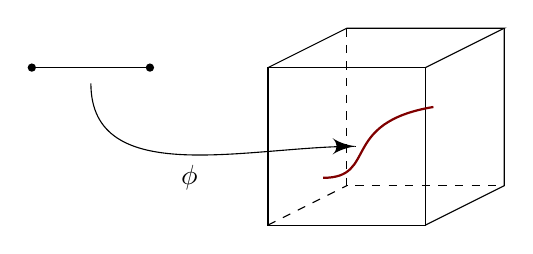
\begin{tikzpicture}
        \draw (0, 0) node [circ] {} -- (1.5, 0) node [circ] {};

        \draw (3, 0) rectangle (5, -2);
        \draw (3, 0) -- (4, 0.5) -- (6, 0.5) -- (5, 0);
        \draw (6, 0.5) -- (6, -1.5) -- (5, -2);
        \draw [dashed] (4, 0.5) -- (4, -1.5) -- (6, -1.5);
        \draw [dashed] (3, -2) -- (4, -1.5);

        \draw (0.75, -0.2) edge [out=270, in=180] (4.1, -1);

        \node at (2, -1.4) {$\phi$};

        \draw [->] (4.099, -1) -- (4.1, -1);

        \draw [thick, mred](3.7, -1.4) .. controls (4.4, -1.4) and (3.9, -0.7) .. (5.1, -0.5);
      \end{tikzpicture}
    \end{center}
    In string theory, we often have fields $\phi: \Sigma \to N$, where $N$ is a \emph{Calabi-Yau manifold}.

    In pion physics, $\pi(x)$ describes a map $\phi: (\R^4, \eta) \to G/H$, where $G$ and $H$ are Lie groups.

    Of course, we can go beyond scalar fields. We can also have fields with non-zero spin such as fermions or gauge fields, eg. a connection on a principal $G$-bundle, as we will figure out later. These are fields that carry a non-trivial representation of the Lorentz group. There is a whole load of things we can choose for our field.

    Whatever field we choose, we let $\mathcal{C}$\index{$\mathcal{C}$} be the space of all field configurations, ie. a point $\phi \in \mathcal{C}$ represents a picture of our field across all of $M$. Thus $\mathcal{C}$ is some form of function space and will typically be infinite dimensional. This infinite-dimensionality is what makes QFT hard, and also what makes it interesting.

  \item We choose an action. An \emph{action} is just a function $S: \mathcal{C} \to \R$. You tell me what the field looks like, and I will give you a number, the value of the action. We often choose our action to be local, in the sense that we assume there exists some function $\mathcal{L}(\phi, \partial \phi, \cdots)$ such that
    \[
      S[\phi] = \int_M\d^4 x \sqrt{g}\; \mathcal{L}(\phi(x), \partial\phi (x), \cdots).
    \]
    The physics motivation behind this choice is obvious --- we don't want what is happening over here to depend on what is happening at the far side of Pluto. However, this assumption is actually rather suspicious, and we will revisit this later.

    For example, we have certainly met actions that look like
    \[
      S[\phi] = \int \d^4 x\; \left(\frac{1}{2} (\partial \phi)^2 + \frac{m^2}{2} \phi^2 + \frac{\lambda}{4!} \phi^4\right),
    \]
    and for gauge fields we might have seen
    \[
      S[A] = \frac{1}{4} \int \d^4 x\; F_{\mu\nu}F^{\mu\nu}.
    \]
    If we have a coupled fermion field, we might have
    \[
      S[A, \psi] = \frac{1}{4} \int \d^4 x\; F_{\mu\nu}F^{\mu\nu} + \bar\psi (\slashed{D} + m) \psi.
    \]
    But recall when we first encountered Lagrangians in classical dynamics, we worked with \emph{lots} of different Lagrangians. We can do whatever thing we like, make the particle roll down the hill and jump into space etc, and we get to deal with a whole family of different Lagrangians. But when we come to quantum field theory, the choices seem to be rather restrictive. Why can't we choose something like
    \[
      S[A] = \int F^2 + F^4 + \cosh(F^2) + \cdots?
    \]
    It turns out we can, and in fact we \emph{must}. We will have to work with something much more complicated.

    But then what were we doing in the QFT course? Did we just waste time coming up with tools that just work with these very specific examples? It turns out not. We will see that there are very good reasons to study these specific actions.
  \item What do we compute? In this course, the main object we'll study is the \term{partition function}
    \[
      \mathcal{Z} = \int_\mathcal{C} \D \phi\; e^{-S[\phi]/\hbar},
    \]
    which is some sort of integral over the space of all fields. Note that the minus sign in the exponential is for the Euclidean signature. If we are not Euclidean, we get some $i$'s instead.

    We will see that the factor of $e^{-S[\phi]/\hbar}$ means that as $\hbar \to 0$, the dominant contribution to the partition function comes from stationary points of $S[\phi]$ over $\mathcal{C}$, and this starts to bring us back to the classical theory of fields. The effect of $e^{-S[\phi]/\hbar}$ is to try to suppress ``wild'' contributions to $\mathcal{Z}$, eg. where $\phi$ is varying very rapidly or $\phi$ takes very large values.

     Heuristically, just as in statistical physics, we have a competition between the two factors $\D \phi$ and $e^{-S[\phi]/\hbar}$. The action part tries to suppress crazy things, but how well this happens depends on how much crazy things are happening, which is measured by the measure $\D \phi$. We can think of this $\D \phi$ as ``entropy''. However, the problem is, the measure $\D \phi$ on $\mathcal{C}$ doesn't actually exist!

    Understanding what we mean by this path integral, and what this measure actually is, and how we can actually compute this thing, and how this has got to do with the canonical quantization operators we had previously, is the main focus of the first part of this course.
\end{enumerate}

\section{QFT in zero dimensions}
We start from the simplest case we can think of, namely quantum field theory in zero dimensions. You might think this is rather trivial, and it is. And this is good.

In $d = 0$, if our universe $M$ is connected, then the only choice of $M$ is $\{\mathrm{pt}\}$. There is a no possibility for a field to have spin, because the Lorentz group is trivial. Our fields are scalar, and the simplest choice is just a single field $\phi: \{\mathrm{pt}\} \to \R$, ie. just a real variable. Similarly, we simply have $\mathcal{C} \cong \R$. This is \emph{not} an infinite-dimensional space.

The action is just a normal function $S: \mathcal{C} \cong \R \to \R$ of one real variable. The path integral measure $\D \phi$ can be taken to just be the standard (Lebesgue) measure $\d \phi$ on $\R$. So our partition function is just
\[
  \mathcal{Z} = \int_\R \d \phi\; e^{-S(\phi)/\hbar},
\]
where we assume $S$ is chosen so that this converges. This happens if $S$ grows sufficiently large as $\phi \to \pm \infty$.

More generally, we may wish to compute \term{correlation functions}, ie. we pick another function $f(\phi)$ and compute the \term{expectation}\index{$\bra f(\phi)\ket$}
\[
  \bra f(\phi)\ket = \frac{1}{\mathcal{Z}} \int \d \phi\; f(\phi) e^{-S(\phi)/\hbar}.
\]
Again, we can pick whatever $f$ we like as long as the integral converges. In this case, $\frac{1}{\mathcal{Z}} e^{-S(\phi)/\hbar}$ is a probability distribution on $\R$, and as the name suggests, $\bra f(\phi)\ket$ is just the expectation value of $f$ in this distribution. Later on, when we study quantum field theory in higher dimensions, we can define more complicated $f$ by evaluating $\phi$ at different points, and we can use this to figure out how the field at different points relate to each other.

Our action is taken to have a series expansion in $\phi$, so in particular we can write
\[
  S(\phi) = \frac{m^2 \phi^2}{2} + \sum_{n = 3}^N g_n \frac{\phi^n}{n!}.
\]
We didn't put in a constant term, as it would just give us a constant factor in $\mathcal{Z}$. We could have included linear terms, but we shall not. The important thing is that $N$ has to be even, so that the asymptotic behaviour of $S$ is symmetric in both sides.

Now the partition function is a function of all these terms: $\mathcal{Z} = \mathcal{Z}(m^2, g_n)$. Similarly, $\bra f\ket$ is again a function of $m^2$ and $g_n$, and possibly other things used to define $f$ itself.

Note that \emph{nothing} depends on the field, because we are integrating over all possible fields.

\subsection{Free theories}
We consider the simplest possible QFT. These QFT's are free, and so $S(\phi)$ is at most quadratic. Classically, this implies the equations of motions are linear, and so there is superposition, and thus the particles do not interact.

Let $\phi: \{\mathrm{pt}\} \to \R^n$ be a field with coordinates $\phi^a$, and define
\[
  S(\phi) = \frac{1}{2} M(\phi, \phi) = \frac{1}{2} M_{ab} \phi^a \phi^b,
\]
where $M: \R^n \times \R^n \to \R$ is a positive-definite symmetric matrix. Then the partition function $\mathcal{Z}(M)$ is just a Gaussian integral:
\[
  \mathcal{Z}(M) = \int_{\R^n} \d^n \phi\; e^{- \frac{1}{2\hbar} M(\phi, \phi)} = \frac{(2 \pi \hbar)^{n/2}}{\sqrt{\det{M}}}.
\]
Indeed, to compute this integral, since $M$ is symmetric, there exists an orthogonal transformation $O: \R^n \to \R^n$ that diagonalizes it. The measure $\d^n \phi$ is invariant under orthogonal transformations. So in terms of the eigenvectors of $M$, this just reduces to a product of $n$ 1D Gaussian integrals of this type, and this is a standard integral:
\[
  \int \d \chi e^{-m\chi^2/2\hbar} = \sqrt{\frac{2\pi \hbar}{m}}.
\]
In our case, $m > 0$ runs over all eigenvalues of $M$, and the product of eigenvalues is exactly $\det M$.

A small generalization is useful. We let
\[
  S(\phi) = \frac{1}{2} M(\phi, \phi) + J(\phi),
\]
where $J: \R^n \to \R$ is some linear map (we can think of $J$ as a (co)vector, and also write $J(\phi) = J \cdot \phi$). $J$ is a \emph{source} in the classical case. Then in this theory, we have
\[
  \mathcal{Z}(M, J) = \int_{\R^n} \d^n \phi\; \exp\left(-\frac{1}{\hbar}\left(\frac{1}{2} M(\phi, \phi) + J(\phi)\right)\right).
\]
To do this integral, we complete the square by letting $\tilde{\phi} = \phi + M^{-1}J$. In other words,
\[
  \tilde{\phi}^a = \phi^a + (M^{-1})^{ab} J_b.
\]
The inverse exists because $M$ is assumed to be positive definite. We can now complete the square to find
\begin{align*}
  \mathcal{Z}(M, J) &= \int_{\R^n} \d^n \tilde{\phi} \;\exp\left(\frac{-1}{2\hbar}M(\tilde{\phi}, \tilde{\phi}) + \frac{1}{2\hbar}M^{-1}(J, J)\right)\\
  &= \exp\left(\frac{1}{2\hbar}M^{-1}(J, J)\right)\int_{\R^n} \d^n \tilde{\phi} \;\exp\left(\frac{-1}{2\hbar}M(\tilde{\phi}, \tilde{\phi})\right)\\
  &= \exp\left(\frac{1}{2\hbar}M^{-1}(J, J)\right) \frac{(2\pi \hbar)^{n/2}}{\sqrt{\det M}}.
\end{align*}
In the long run, we really don't care about the case with a source. However, we will use this general case to compute some correlation functions.

We return to the case without a source, and let $P: \R^n \to \R$ be a polynomial. We want to compute
\[
  \bra P(\phi)\ket = \frac{1}{\mathcal{Z}(M)} \int_{\R^n} \d^n \phi\; P(\phi) \exp\left(-\frac{1}{2\hbar} M(\phi, \phi)\right).
\]
By linearity, it suffices to consider the case where $P$ is just a monomial, so
\[
  P(\phi) = \prod_{i = 1}^m (\ell_i(\phi)),
\]
for $\ell_i : \R^n \to \R$ linear maps. Now if $m$ is odd, then clearly $\bra P(\phi)\ket = 0$, since this is an integral of an odd function. When $m = 2k$, then we have
\[
  \bra P(\phi) \ket = \frac{1}{\mathcal{Z}(M)} \int \d^n \phi\; (\ell_i\cdot \phi) \cdots (\ell_{2k} \cdot \phi) \exp\left(-\frac{1}{2\hbar}M (\phi, \phi) - \frac{J \cdot \phi}{\hbar}\right).
\]
Here we are eventually going to set $J = 0$, but for the time being, we will be silly and put the source there. The relevance is that we can then think of our factors $\ell_i \cdot \phi$ as derivatives with respect to $J$:
\begin{align*}
  \bra P(\phi)\ket &= \frac{(-\hbar)^{2k}}{\mathcal{Z}(M)} \int \d^n \phi \; \prod_{i = 1}^{2k} \left(\ell_i \cdot \frac{\partial}{\partial J}\right) \exp\left(-\frac{1}{2\hbar} M(\phi, \phi) - \frac{J\cdot \phi}{\hbar}\right)\\
  \intertext{Since the integral is absolutely convergent, we can move the derivative out of the integral, and get}
  &= \frac{(-\hbar)^{2k}}{\mathcal{Z}(M)} \prod_{i = 1}^{2k} \left(\ell_i \cdot \frac{\partial}{\partial J}\right) \int \d^n \phi \; \exp\left(-\frac{1}{2\hbar} M(\phi, \phi) - \frac{J\cdot \phi}{\hbar}\right)\\
  &= \hbar^{2k} \prod_{i = 1}^{2k} \left(\ell_i \cdot \frac{\partial}{\partial J}\right) \exp\left(\frac{1}{2\hbar}M^{-1}(J, J)\right).
\end{align*}
When each derivative $\ell_i \cdot \frac{\partial}{\partial J}$ acts on the exponential, we obtain a factor of
\[
  \frac{1}{\hbar} M^{-1}(J, \ell_i).
\]
in front. At the end, we are going to set $J = 0$. So we only get contributions if and only if exactly half (ie. $k$) of the derivatives act on the exponential, and the other $k$ act on the factor in front to get rid of the $J$.

We let $\sigma$ denote a (complete) pairing of the set $\{1, \cdots, 2k\}$, and $\Pi_{2k}$ be the set of all such pairings. For example, if we have $k = 2$, then the possible pairings are $\{(1, 2), (3, 4)\}$, $\{(1, 3), (2, 4)\}$ and $\{(1, 4), (2, 3)\}$:
\begin{center}
  \begin{tikzpicture}
    \node [circ] at (0, 0) {};
    \node [circ] at (1, 0) {};
    \node [circ] at (1, 1) {};
    \node [circ] at (0, 1) {};
    \draw (0, 0) -- (0, 1);
    \draw (1, 0) -- (1, 1);

    \begin{scope}[shift={(3, 0)}]
      \node [circ] at (0, 0) {};
      \node [circ] at (1, 0) {};
      \node [circ] at (1, 1) {};
      \node [circ] at (0, 1) {};
      \draw (0, 0) -- (1, 0);
      \draw (0, 1) -- (1, 1);
    \end{scope}

    \begin{scope}[shift={(6, 0)}]
      \node [circ] at (0, 0) {};
      \node [circ] at (1, 0) {};
      \node [circ] at (1, 1) {};
      \node [circ] at (0, 1) {};
      \draw (0, 0) -- (1, 1);
      \draw (1, 0) -- (0, 1);
    \end{scope}
  \end{tikzpicture}
\end{center}
In general, we have
\[
  |\Pi_{2k}| = \frac{(2k)!}{2^k k!},
\]
and we have
\begin{thm}[Wick's theorem]\index{Wick's theorem}
  For a monomial
  \[
    P(\phi) = \prod_{i = 1}^{2k} \ell_i(\phi),
  \]
  we have
  \[
    \bra P(\phi)\ket = \hbar^{k}\sum_{\sigma \in \Pi_{2k}} \prod_{i \in \{1, \cdots, 2k\}/\sigma} M^{-1}(\ell_i, \ell_{\sigma(i)}).
  \]
  where the $\{1, \cdots, 2k\}/\sigma$ says we sum over each pair $\{i, \sigma(i)\}$ only once, rather than once for $(i, \sigma(i))$ and another for $(\sigma(i), i)$.
\end{thm}
This is in fact the version of Wick's theorem for this 0d QFT, and $M^{-1}$ plays the role of the propagator.

For example, we have
\[
  \bra \ell_1(\phi), \ell_2(\phi)\ket = \hbar M^{-1} (\ell_1, \ell_2).
\]
We can represent this by the diagram
\begin{center}
  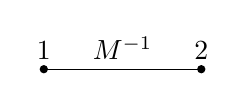
\begin{tikzpicture}
    \node [circ] at (0, 0) {};
    \node [circ] at (2, 0) {};

    \node [above] at (0, 0) {$1$};
    \node [above] at (2, 0) {$2$};
    \draw (0, 0) -- (2, 0) node [pos=0.5, above] {$M^{-1}$};
  \end{tikzpicture}
\end{center}
Similarly, we have
\begin{multline*}
  \bra \ell_1(\phi) \cdots \ell_4(\phi)\ket = \hbar^2 \Big(M^{-1}(\ell_1, \ell_2) M^{-1}(\ell_3, \ell_4) \\
  + M^{-1}(\ell_1, \ell_3) M^{-1}(\ell_2, \ell_4) + M^{-1}(\ell_1, \ell_4) M^{-1}(\ell_2, \ell_3)\Big).
\end{multline*}
This is purely combinatorial.

This is about all we can say for free 0d QFTs. There is an analogue for ``fermions'', which is put in the first example sheet.

\subsection{Interacting theories}
Physically interesting theories contain interactions, ie. $S(\phi)$ is non-quadratic. Typically, if we are trying to compute
\[
  \int \d^n \phi P(\phi) \exp\left(-\frac{S(\phi)}{\hbar}\right),
\]
these things involve transcendental functions and, except in very special circumstances, is just too hard. We usually cannot perform these integrals analytically.

Naturally, in perturbation theory, we would thus want to approximate
\[
  \mathcal{Z} = \int \d^n \phi\; \exp\left(-\frac{S(\phi)}{\hbar}\right)
\]
by some series. Unfortunately, the integral very likely diverges if $\hbar < 0$, as usually $S(\phi) \to \infty$ as $\phi \to \pm\infty$. So it can't have a Taylor series expansion around $\hbar = 0$, as such expansions have to be valid in a disk in the complex plane. The best we can hope for is an asymptotic series.

Recall that a series
\[
  \sum_{n = 0}^\infty f_n(\hbar)
\]
is an \emph{asymptotic series} for $\mathcal{Z}(\hbar)$ if for any fixed $N \in \N$, if we write $\mathcal{Z}_N(\hbar)$ for the first $N$ terms on the RHS, then
\[
  \lim_{\hbar \to 0^+} \frac{|\mathcal{Z}(\hbar) - \mathcal{Z}_N(\hbar)|}{\hbar^N} \to 0.
\]
Thus as $\hbar \to 0^+$, we get an arbitrarily good approximation to what we really wanted from any finite number of terms. But the series will in general diverge if try to fix $\hbar \in \R_{> 0}$, and include increasingly many terms.

Most of the expansions we do in quantum field theories are of this nature.

Now suppose $S(\phi)$ is smooth with a global minimum at $\phi = \phi_0 \in \R^n$, where the Hessian
\[
  \left.\frac{\partial^2 S}{\partial \phi^a \partial \phi^b}\right|_{\phi_0}
\]
is positive definite. Then by Laplace's method/Watson's lemma, we have an asymptotic series of the form
\[
  \mathcal{Z}(\hbar) \sim (2\pi \hbar)^{n/2} \frac{\exp\left(-\frac{S(\phi_0)}{\hbar}\right)}{\sqrt{\det \partial_a \partial_b S(\phi_0)}} \left(1 + A \hbar + B \hbar^2 + \cdots\right).
\]
We will not prove this, but the proof is available in any standard asymptotic methods textbook. The leading term involves the action evaluated on the classical solution $\phi_0$, and is known as the \term{semiclassical term}. Every thing we did last term with tree diagrams was about calculating the first term. The remaining terms are called the \term{quantum correction}.

In Quantum Field Theory last term, the tree diagrams we worked with were just about calculating the leading term. So we weren't actually doing \emph{quantum} field theory (sorry).

\begin{eg}
  Let's consider a single scalar field $\phi$ with action
  \[
    S(\phi) = \frac{m^2}{2}\phi^2 + \frac{\lambda}{4!} \phi^4,
  \]
  where $m^2, \lambda > 0$. The action has a unique global minimum at $\phi_0 = 0$. The action evaluated at $\phi_0 = 0$ vanishes, and $\partial^2 S/\hbar = m^2$. So the leading term in the asymptotic expansion of $\mathcal{Z}(\hbar, m \lambda)$ is
  \[
    \frac{(2\pi \hbar)^{1/2}}{m}.
  \]
  Further, we can find the whole series expansion by
  \begin{align*}
    \mathcal{Z}(\hbar, m, \lambda) &= \int_\R \d \phi \; \exp\left(\frac{-1}{\hbar}\left(\frac{m^2}{2} \phi^2 + \frac{\lambda}{4!}\phi^4\right)\right)\\
    &= \frac{\sqrt{2\hbar}}{m} \int \d \tilde{\phi} \exp\left(-\tilde{\phi}^2 \right) \exp\left( - \frac{4\lambda \hbar}{4! m^4} \tilde{\phi}^4\right)\\
    &\sim \frac{\sqrt{2\hbar}}{m} \int \d \tilde{\phi}\; e^{- \tilde{\phi}^2}\sum_{n = 0}^N \frac{1}{n!} \left(\frac{-\lambda \hbar}{3! m^4}\right)^n \tilde{\phi}^{4n}\\
    &= \frac{\sqrt{2\hbar}}{m} \sum_{n = 0}^N \left(\frac{-\lambda \hbar}{3! m^4}\right)^n \frac{1}{n!} \int \d \tilde{\phi}\;e^{- \tilde{\phi}^2}\tilde{\phi}^{4n}\\
    &= \frac{\sqrt{2\hbar}}{m} \sum_{n = 0}^N \left(\frac{-\lambda \hbar}{3! m^4}\right)^n \frac{1}{n!} \Gamma\left(2n + \frac{1}{2}\right).
  \end{align*}
  The last line uses the definition of the Gamma function.

  We can plug in the value of the $\Gamma$ function to get
  \begin{align*}
    \mathcal{Z}(\hbar, m \lambda) &\sim \frac{\sqrt{2\hbar \pi}}{m} \sum_{n = 0}^N \left(\frac{-\hbar \lambda}{m^4}\right)^n \frac{1}{(4!)^n n!} \frac{(4n)!}{4^n (2n)!}\\
    &= \frac{\sqrt{2\pi \hbar}}{m} \left(1 - \frac{\hbar\lambda}{8m^4} + \frac{35}{384} \frac{\hbar^2 \lambda^2}{m^8} + \cdots\right).
  \end{align*}
  We will get to understand these coefficients much more in terms of Feynman diagrams later.

  Note that up to the factor $\frac{\sqrt{2\pi \hbar}}{m}$, the series depends on $(\hbar, \lambda)$ only through the product $\hbar \lambda$. So we can equally view it as an asymptotic series in the coupling constant $\lambda$.
\end{eg}
As we emphasized previously, we get an asymptotic series, not a Taylor series. Why is this so?

When we first started our series expansion, we wrote $\exp(-S(\phi)/\hbar)$ as a series in $\lambda$. This is absolutely fine, as $\exp$ is a very well-behaved function when it comes to power series. The problem comes when we want to interchange the integral with the sum. We know this is allowed only if the sum is absolutely convergent, but it is not, as the integral does not converge for negative $\hbar$. Thus, the best we can do is that for any $N$, we truncate the sum at $N$, and then do the exchange. This is legal since finite sums always commute with integrals.

We can in fact see the divergence of the asymptotic series for finite $(\hbar \lambda) > 0$ from the series itself, using Stirling's approximation. Recall we have
\[
  n! \sim e^{n \log n}.
\]
So via a straightforward manipulation, we have
\[
  \frac{1}{(4!)^n n!} \frac{(4n)!}{4^n(2n)!} \sim e^{n \log n}.
\]
So the coefficients go faster than exponentially, and thus the series has vanishing radius of convergence.

We can also see other weird phenomena here. Suppose we decided that we have $m^2 < 0$ instead (which is a rather weird thing to do). Then it is clear that $\mathcal{Z}(m^2, \lambda)$ still exists, as the $\phi^4$ eventually dominates, and so what happens at the $\phi^2$ term doesn't really matter. However, the asymptotic series is invalid in this region.

Indeed, if we look at the fourth line of our derivation, each term in the asymptotic series will be obtained by integrating $e^{\tilde\phi^2} \tilde\phi^{4n}$, instead of integrating $e^{-\tilde\phi^2} \tilde\phi^{4n}$, and each of these integrals would diverge.

Fundamentally, this is since when $m^2 < 0$, the global minimum of $S(\phi)$ are now at
\[
  \phi_0 = \pm \sqrt{\frac{6m^2}{\lambda}}.
\]
\begin{center}
  \begin{tikzpicture}
    \draw [->](-3, 0) -- (3, 0) node [right] {$\phi$};
    \draw [->] (0, -1.2) -- (0, 3) node [above] {$S(\phi)$};

    \draw [mblue, thick, domain=-2.4:2.4, samples=50] plot [smooth] (\x, {4 * ((\x/2)^4 - (\x/2)^2)});

    \draw [dashed] (1.414, 0) node [above] {$\phi_0$} -- (1.414, -1);
  \end{tikzpicture}
\end{center}
Our old minimum $\phi = 0$ is now a (local) maximum!T This is the wrong point to expand about! Fields with $m^2 < 0$ are called \term{tachyons}, and these are always signs of some form of instability.

Actions whose minima occur at non-zero field values are often associated with \term{spontaneous symmetry breaking}. Our original theory has a $\Z/2$ symmetry, namely under the transformation $x \leftrightarrow -x$. But once we pick a minimum $\phi_0$ to expand about, we have broken the symmetry. This is an interesting kind of symmetry breaking because the asymmetry doesn't really exist in our theory. It's just our arbitrary choice that breaks it.

\subsection{Feynman diagrams}
We now try to understand the terms in the asymptotic series in terms of Feynman diagrams. The easy bits are the powers of
\[
  \left(\frac{\hbar \lambda}{m^4}\right)^n.
\]
This combination is essentially fixed by dimensional analysis. What we really want to understand are the combinatorial factors, given by
\[
  \frac{1}{(4!)^n n!} \times \frac{(4n)!}{4^n (2n)!}.
\]
The first factor just came from expanding $\exp(-\lambda \phi^4/4!)$ in the exponential. The second term is more interesting. It is the number of ways of joining $4n$ elements into inequivalent pairs. This is something we saw when we looked at Wick's theorem. We have $4n$ instead of $2n$ because we are now doing perturbation theory with $\phi^4$, not $\phi^2$.

We now try to come up with some Feynman diagrams to represent our asymptotic series. We have a single type of propagator that looks like this:
\begin{center}
  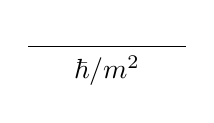
\begin{tikzpicture}
    \draw (0, 0) -- (2, 0) node [pos=0.5, below] {$\hbar/m^2$} node [pos=0.5, above] { };
  \end{tikzpicture}
\end{center}
and we also have a vertex
\begin{center}
  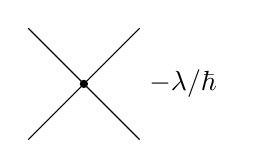
\begin{tikzpicture}[scale=0.707]
    \draw (0, 0) -- (2, 2);
    \draw (0, 2) -- (2, 0);
    \node [circ] at (1, 1) {};
    \node [right] at (2, 1) {$-\lambda /\hbar$};
  \end{tikzpicture}
\end{center}
The negative sign appears because we have $e^{-S}$ in ``Euclidean'' QFT.

Since we are computing just the partition functions, we want to try to find all \term{vacuum graphs}, ie. graphs with no external edges. The only allowed components are the propagator and vertices.

At order $\lambda$, we have
\begin{center}
  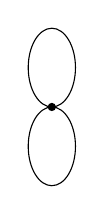
\begin{tikzpicture}
    \node [circ] at (0, 0) {};

    \draw (0, 0.5) ellipse (0.3 and 0.5);
    \draw (0, -0.5) ellipse (0.3 and 0.5);
  \end{tikzpicture}
\end{center}
For our purposes, it is useful to consider the four outgoing vertices of the diagram as sort-of distinct. So the following can be considered different diagrams:
\begin{center}
  \makecenter{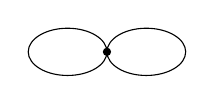
\begin{tikzpicture}
    \node [circ] at (0, 0) {};

    \draw (0.5, 0) ellipse (0.5 and 0.3);
    \draw (-0.5, 0) ellipse (0.5 and 0.3);
  \end{tikzpicture}}
  \quad
  \makecenter{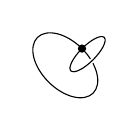
\begin{tikzpicture}[rotate=135]
    \draw (0, 0.3) ellipse (0.5 and 0.3);
    \draw [ultra thick, white] (-0.1, 0) ellipse (0.1 and 0.3);
    \draw (-0.1, 0) ellipse (0.1 and 0.3);

    \node [circ] at (0, 0) {};
  \end{tikzpicture}}
\end{center}
However, we will say these are \emph{topologically equivalent}. In the future, we will count these as the ``same'' diagram, and only include them once in the series expansion, but we will later see the need to distinguish between them when we want to figure out how many times we count each diagram.

In terms of these diagrams, we can write
\[\arraycolsep=0.25em\def\arraystretch{2.2}
  \begin{array}{ccccccccccccc}
  \displaystyle\frac{\mathcal{Z}(m^2, \lambda)}{\mathcal{Z}(m^2, 0)} & \sim &
  \begin{tikzpicture}[eqpic]
    \node {$\emptyset$};
  \end{tikzpicture} &+&
  \begin{tikzpicture}[eqpic]
    \node [circ] at (0, 0) {};

    \draw (0, 0.5) ellipse (0.3 and 0.5);
    \draw (0, -0.5) ellipse (0.3 and 0.5);
  \end{tikzpicture}
  &+&
  \begin{tikzpicture}[eqpic]
    \node [circ] at (0, 0) {};
    \node [circ] at (1.5, 0) {};
    \draw (0.75, 0) ellipse (0.75 and 0.7);
    \draw (0.75, 0) ellipse (0.75 and 0.4);
  \end{tikzpicture}
  &+&
  \begin{tikzpicture}[eqpic]
    \node [circ] at (0, 0) {};
    \node [circ] at (1, 0) {};
    \draw (-0.2, 0) ellipse (0.2 and 0.5);
    \draw (0.5, 0) ellipse (0.5 and 0.3);
    \draw (1.2, 0) ellipse (0.2 and 0.5);
  \end{tikzpicture}
  &+&
  \begin{tikzpicture}[eqpic]
    \node [circ] at (0, 0) {};

    \draw (0, 0.5) ellipse (0.3 and 0.5);
    \draw (0, -0.5) ellipse (0.3 and 0.5);

    \node [circ] at (0.7, 0) {};

    \draw (0.7, 0.5) ellipse (0.3 and 0.5);
    \draw (0.7, -0.5) ellipse (0.3 and 0.5);
  \end{tikzpicture}
  &+&
  \cdots\\
  && 1 &+& \displaystyle\frac{-\lambda \hbar}{m^4} \frac{1}{8} &+& \displaystyle\frac{\lambda^2 \hbar^2}{m^8} \frac{1}{48} &+& \displaystyle\frac{\lambda^2 \hbar^2}{m^8} \frac{1}{16} &+& \displaystyle\frac{\lambda^2 \hbar^2}{m^8} \frac{1}{128} &+& \cdots
\end{array}
\]
The $\lambda, \hbar$ and $m$ factors just come directly form the Feynman rules, but where did the numerical factors come from?

Let $D_n$ be the set of all Feynman graphs with $n$ vertices. By some combinatorics, we find that there are
\[
  |D_n| = \frac{(4n)!}{4^n (2n)!}
\]
of these. For example, $|D_1| = 3$, as we have previously seen listed.

This set $D_n$ is acted on by a group $G_n = (S_4)^n \rtimes S_n$, where $S_4$ permutes the $4$ loops on a given vertex, and $S_n$ permutes the different vertices. The order of this group is
\[
  |G_n| = (4!)^n n!
\]
Then we see that our asymptotic series can be written as
\[
  \frac{\mathcal{Z}(m^2, \lambda)}{\mathcal{Z}(m^2, 0)} \sim \sum_{n = 0}^N \frac{|D_n|}{|G_n|} \left(\frac{-\hbar \lambda}{m^4}\right)^n.
\]
Now we just gave names to these numbers, and it doesn't help us actually compute them from Feynman diagrams. To make more sense of these numbers, we need to use the renowned \emph{orbit-stabilizer theorem} we learnt from IA Groups.

Note that when $G_n$ acts on $D_n$, the action does not change the topology of the graph, ie. after the action of $G_n$, the graph is still topologically equivalent to the original one. In particular, the set of \term{orbits} $\mathcal{O}_N$ of $D_n$ under the $G_n$-action are exactly the topologically distinct graphs.

For example, we have $|\mathcal{O}_1| = 1$ and $|\mathcal{O}_2| = 3$.

Now we fix a particular element $\Gamma \in G_n$, and pick one particular graph that represents $\Gamma$, say
\begin{center}
  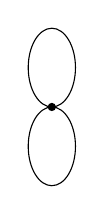
\begin{tikzpicture}
    \node [circ] at (0, 0) {};

    \draw (0, 0.5) ellipse (0.3 and 0.5);
    \draw (0, -0.5) ellipse (0.3 and 0.5);
  \end{tikzpicture}
\end{center}
Now if we swap the two top legs, then we get back the same graph. However, if we swap the top-right and bottom-left legs, we end up with
\begin{center}
  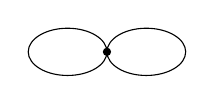
\begin{tikzpicture}
    \node [circ] at (0, 0) {};

    \draw (0.5, 0) ellipse (0.5 and 0.3);
    \draw (-0.5, 0) ellipse (0.5 and 0.3);
  \end{tikzpicture}
\end{center}
We write $\Aut \Gamma$ for the set (and in fact subgroup) of all elements in $G_n$ that preserve the graph. It is an easy exercise to show this does not depend which representative of $\Gamma$ we pick. This is known as the \term{stabilizer} of $\Gamma$.

Now by the \term{orbit-stabilizer theorem}, we know
\[
  \frac{|D_n|}{|G_n|} = \sum_{\Gamma \in \mathcal{O}_n} \frac{1}{|\Aut\Gamma|}.
\]
For example, in $n = 1$, the graph
\begin{center}
  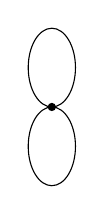
\begin{tikzpicture}
    \node [circ] at (0, 0) {};

    \draw (0, 0.5) ellipse (0.3 and 0.5);
    \draw (0, -0.5) ellipse (0.3 and 0.5);
  \end{tikzpicture}
\end{center}
has stabilizer of size $8$. This is generated by swapping the top legs; swapping the bottom legs; and a vertical flip.

In $n = 2$, the graph
\begin{center}
  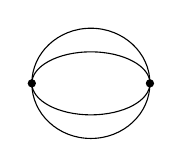
\begin{tikzpicture}
    \node [circ] at (0, 0) {};
    \node [circ] at (1.5, 0) {};
    \draw (0.75, 0) ellipse (0.75 and 0.7);
    \draw (0.75, 0) ellipse (0.75 and 0.4);
  \end{tikzpicture}
\end{center}
has $|\Aut \Gamma| = 4! \times 2 = 48$, as we can permute any of the edges, giving a factor of $4!$, and we can also swap around the two vertices.

In
\begin{center}
  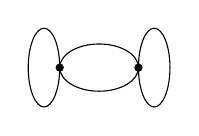
\begin{tikzpicture}
    \node [circ] at (0, 0) {};
    \node [circ] at (1, 0) {};
    \draw (-0.2, 0) ellipse (0.2 and 0.5);
    \draw (0.5, 0) ellipse (0.5 and 0.3);
    \draw (1.2, 0) ellipse (0.2 and 0.5);
  \end{tikzpicture}
\end{center}
we have $|\Aut\Gamma| = 2^3 \times 2 = 16$, as we can flip the left; middle; or right loops, giving $2^3$, and also we can flip the whole thing around horizontally.

Finally, in
\begin{center}
  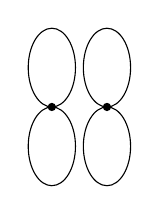
\begin{tikzpicture}
    \node [circ] at (0, 0) {};

    \draw (0, 0.5) ellipse (0.3 and 0.5);
    \draw (0, -0.5) ellipse (0.3 and 0.5);

    \node [circ] at (0.7, 0) {};

    \draw (0.7, 0.5) ellipse (0.3 and 0.5);
    \draw (0.7, -0.5) ellipse (0.3 and 0.5);
  \end{tikzpicture}
\end{center}
we have $|\Aut\Gamma| = 8 \times 8 \times 2 = 128$, as we have $8$ on each individual component, and we can also swap them.

More generally, if we have a theory with several fields with propagators of value $\frac{1}{P_i}$, and many different interactions with coupling constants $\lambda_\alpha$, then
\[
  \frac{\mathcal{Z}(\lambda_\alpha)}{ \mathcal{Z}(0)} = \sum_{n = 0}^N \sum_{\Gamma \in \mathcal{O}_N} \frac{1}{|\Aut \Gamma|} \frac{\prod_\alpha \lambda_\alpha^{|v_\alpha(\Gamma)|}}{\prod_i |P_i|^{|e_i(\Gamma)|}} \hbar^{E(\Gamma) - V(\Gamma)},
\]
where
\begin{itemize}
  \item $e_i(\Gamma)$ is the number of edges of type $i$ in $\Gamma$;
  \item $v_\alpha(\Gamma)$ is the number of vertices of type $\alpha$ in $\Gamma$;
  \item $V(\Gamma)$ is the number of vertices in total; and
  \item $E(\Gamma)$ the total number of edges.
\end{itemize}
But by Euler's theorem, we have $E - V = L - C$, where $L$ is the number of loops in the graph and $C$ is the number of connected components. So we can also write the factor as $\hbar^{L - C}$.

Finally, note that
\[
  \log (\mathcal{Z}/\mathcal{Z}_0)
\]
is the sum of all \emph{connected} graphs. Indeed, we can see that the term for the two-figure-of-eight is just the square of the term for a single figure-of-eight times the factor of $\frac{1}{2!}$, and one can easily convince oneself that this is true for any number of disconnected sums.

In general, A generic QFT has an asymptotic series
\[
  \mathcal{Z}(\hbar) \sim (2\pi \hbar)^{n/2}\frac{e^{-S(\phi_0)/\hbar}}{\sqrt{ \det \partial \partial S|_{\phi_0}}} (1 + a_1 \hbar + a_2 \hbar^2 + \cdots),
\]
and the terms in the series can be computed by Feynman diagrams.

In some special theories, the leading term is the \emph{exact} answer! The tail terms somehow manage to cancel each other out. This happens for supersymmetry theories. We will not go into the exact details.

\subsection{An effective theory}
We now play with another toy theory. Suppose we have two scalar fields $\phi, \chi \in \R$, and consider the action
\[
  S(\phi, \chi) = \frac{m^2}{2}\phi^2 + \frac{M^2}{2} \chi^2 + \frac{\lambda}{4} \phi^2 \chi^2.
\]
Correspondingly, we have Feynman rules
\begin{center}
  \makecenter{
  \begin{tikzpicture}
    \draw (0, 0) -- (2, 0) node [pos=0.5, below] {$1/m^2$} node [pos=0.5, above] { };
  \end{tikzpicture}}\quad\quad
  \makecenter{\begin{tikzpicture}
    \draw [dashed] (0, 0) -- (2, 0) node [pos=0.5, below] {$1/M^2$} node [pos=0.5, above] { };
  \end{tikzpicture}}
\end{center}
with a vertex
\begin{center}
  \begin{tikzpicture}[scale=0.707]
    \draw (0, 0) -- (2, 2);
    \draw [dashed] (0, 2) -- (2, 0);
    \node [circ] at (1, 1) {};
    \node [right] at (2, 1) {$-\lambda$};
  \end{tikzpicture}
\end{center}
We can use these to compute correlation functions and expectation values.
For example, we might want to compute
\[
  \log (\mathcal{Z}/\mathcal{Z}_0).
\]
We have a diagram that looks like
\[\everymath{\displaystyle}\arraycolsep=0.17em\def\arraystretch{2.2}
  \begin{array}{ccccccccccc}
  \displaystyle\log \left(\frac{\mathcal{Z}(m^2, \lambda)}{\mathcal{Z}(m^2, 0)}\right) & \sim &
  \begin{tikzpicture}[eqpic]
    \node [circ] at (0, 0) {};

    \draw [dashed] (0, 0.5) ellipse (0.3 and 0.5);
    \draw (0, -0.5) ellipse (0.3 and 0.5);
  \end{tikzpicture}
  &+&
  \begin{tikzpicture}[eqpic]
    \node [circ] at (0, 0) {};
    \node [circ] at (1, 0) {};
    \draw (-0.2, 0) ellipse (0.2 and 0.5);
    \draw [dashed] (0.5, 0) ellipse (0.5 and 0.3);
    \draw (1.2, 0) ellipse (0.2 and 0.5);
  \end{tikzpicture}
  &+&
  \begin{tikzpicture}[eqpic]
    \node [circ] at (0, 0) {};
    \node [circ] at (1, 0) {};
    \draw [dashed] (-0.2, 0) ellipse (0.2 and 0.5);
    \draw (0.5, 0) ellipse (0.5 and 0.3);
    \draw [dashed] (1.2, 0) ellipse (0.2 and 0.5);
  \end{tikzpicture}
  &+&
  \begin{tikzpicture}[eqpic]
    \node [circ] at (0, 0) {};
    \node [circ] at (1.5, 0) {};
    \draw [dashed] (0.75, 0) ellipse (0.75 and 0.7);
    \draw (0.75, 0) ellipse (0.75 and 0.4);
  \end{tikzpicture}
  &+&
  \cdots\\
  && \frac{-\lambda}{4m^2 M^2} &+& \frac{\lambda^2}{16 m^4 M^4} &+& \frac{\lambda^2}{16 m^4 M^4} &+& \frac{\lambda^2}{8 m^4 M^4} &+& \cdots\\
\end{array}
\]
We can also try to compute $\bra \phi^2\ket$. To do so, we consider diagrams with two vertices connected to a solid line:
\begin{center}
  \begin{tikzpicture}
    \draw (0, 0) node [circ] {} -- (2, 0);
  \end{tikzpicture}
\end{center}
The relevant diagrams are
\[\everymath{\displaystyle}\arraycolsep=0.3em\def\arraystretch{2.2}
  \begin{array}{ccccccccccccc}
  \displaystyle \bra \phi^2 \ket &\sim&
  \begin{tikzpicture}[eqpic]
    \node [circ] at (0, 0) {};
    \node [circ] at (0, -2) {};
    \draw (0, 0) -- (0, -2);
  \end{tikzpicture}
  &+&
  \begin{tikzpicture}[eqpic]
    \node [circ] at (0, 0) {};
    \node [circ] at (0, -2) {};
    \draw (0, 0) -- (0, -2);

    \node [circ] at (0, -1) {};

    \draw [dashed] (0.4, -1) ellipse (0.4 and 0.25);
  \end{tikzpicture}
  &+&
  \begin{tikzpicture}[eqpic]
    \node [circ] at (0, 0) {};
    \node [circ] at (0, -2) {};
    \draw (0, 0) -- (0, -2);

    \node [circ] at (0, -0.667) {};
    \node [circ] at (0, -1.333) {};

    \draw [dashed] (0.4, -0.667) ellipse (0.4 and 0.25);
    \draw [dashed] (0.4, -1.333) ellipse (0.4 and 0.25);
  \end{tikzpicture}
  &+&
  \begin{tikzpicture}[eqpic]
    \node [circ] at (0, 0) {};
    \node [circ] at (0, -2) {};
    \draw (0, 0) -- (0, -2);

    \node [circ] at (0, -0.667) {};
    \node [circ] at (0, -1.333) {};

    \draw [dashed] (0, -1) ellipse (0.333 and 0.333);
  \end{tikzpicture}
  &+&
  \begin{tikzpicture}[eqpic]
    \node [circ] at (0, 0) {};
    \node [circ] at (0, -2) {};
    \draw (0, 0) -- (0, -2);
    \node [circ] at (0, -1) {};

    \draw [dashed] (0.4, -1) ellipse (0.4 and 0.25);
    \node [circ] at (0.8, -1) {};

    \draw (1.2, -1) ellipse (0.4 and 0.25);
  \end{tikzpicture}
  &+&
  \cdots\\
  && \frac{1}{m^2} &+& \frac{-\lambda}{2m^4 M^4} &+& \frac{\lambda^2}{4m^6 M^4} &+& \frac{\lambda^2}{2m^6 M^4} &+& \frac{\lambda^2}{4m^6 M^4} &+& \cdots\\
\end{array}
\]
Let's arrive at this result in a different way. Suppose we think of $\chi$ as ``heavy'', so we cannot access it directly using our experimental equipment. In particular, if we're only interested in the correlation functions that depend only on $\phi$, then we could try to ``integrate out'' $\chi$ first.

Suppose we have a function $f(\phi)$, and consider the integral
\[
  \int_{\R^2} \d \phi\;\d \chi\; f(\phi) e^{-S(\phi, \chi)/\hbar} = \int_\R \d \phi \left(f(\phi) \int_\R \d \chi\;e^{-S(\phi, \chi)/\hbar}\right).
\]
We define the \term{effective action} for $\phi$, $S_{\mathrm{eff}}(\phi)$ by
\[
  S_{\mathrm{eff}}(\phi) = -\hbar \log \left(\int_\R \d \chi e^{-S(\phi, \chi)/\hbar}\right).
\]
Then the above integral becomes
\[
  \int_\R \d \phi\; f(\phi) e^{-S_{\mathrm{eff}}(\phi)/\hbar}.
\]
So doing any computation with $\phi$ only is equivalent to pretending $\chi$ doesn't exist, and using this effective potential instead.


In general, the integral is very difficult to compute, and we can only find an asymptotic series for the effective action. However, in this very particular example, we have chosen $S$ such that it is only quadratic in $\chi$, and one can compute to get
\[
  \int_\R \d \chi\; e^{-S(\phi, \chi)/\hbar} = e^{-m^2 \phi^2/2\hbar} \sqrt{\frac{2\pi \hbar}{M^2 + \lambda \phi^2/2}}.
\]
Therefore we have
\begin{align*}
  S_{\mathrm{eff}}(\phi) &= \frac{m^2}{2}\phi^2 + \frac{\hbar}{2} \log \left(1 + \frac{\lambda \phi^2}{2M^2}\right) + \frac{\hbar}{2} \log \left(\frac{M^2}{2\pi \hbar}\right)\\
  &= \left(\frac{m^2}{2} + \frac{\hbar \lambda}{4M^2}\right)\phi^2 - \frac{\hbar \lambda^2}{16 M^4} \phi^4 + \frac{\hbar \lambda^3}{48 M^6} \phi^6 + \cdots + \frac{\hbar}{2} \log \left(\frac{M^2}{2\pi \hbar}\right)\\
  &= \frac{m_{\mathrm{eff}}^2}{2} \phi^2 + \frac{\lambda_4}{4!} \phi^4 + \frac{\lambda_6}{6!} \phi^6 + \cdots + \frac{\hbar}{2} \log \left(\frac{M^2}{2\pi \hbar}\right),
\end{align*}
where
\[
  \lambda_{2k} = (-1)^{k + 1} \frac{\hbar (2k)!}{2^{k + 1}k!} \frac{\lambda^k}{M^{2k}}.
\]
We see that once we integrated out $\chi$, we have generated an \emph{infinite series} of new interactions for $\phi$ in $S_{\mathrm{eff}} (\phi)$. Moreover, the mass also shifted as
\[
  m^2 \mapsto m^2_{\mathrm{eff}} = m^2 + \frac{\hbar \lambda}{2M^4}.
\]
Notice the new vertices generated are \emph{quantum effects}. They vanish as $\hbar \to 0$ (they happen to be linear in $\hbar$ here, but that is just a coincidence). They are also suppressed by powers of $\frac{1}{M^2}$. So if $\chi$ is very very heavy, we might think these new couplings have very tiny effects.

This is a very useful technique. If the universe is very complicated with particles at very high energies, then it would be rather hopeless to try to account for all of the effects of the particles we cannot see. In fact, it is impossible to know about these very high energy particles, as their energy are too hight to reach. All we can know about them is their incarnation in terms of these induced couplings on lower energy fields.

A few things to note:
\begin{itemize}
  \item The original action had a $\Z_2 \times \Z_2$ symmetry, given by $(\phi, \chi) \mapsto (\pm \phi, \pm \chi)$. This symmetry is preserved, and we do not generate any vertices with odd powers of $\phi$.
  \item The field $S_{\mathrm{eff}}(\phi)$ also contains a field independent term
    \[
      \frac{\hbar}{2} \log \left(\frac{M^2}{2\pi \hbar}\right).
    \]
    This plays no role in correlation functions $\bar f(\phi)\ket$. Typically, we are just going to drop it. However, this is one of the biggest problem in physics. This term contributes to the cosmological constant, and the values we typically obtain is much larger than the actual observed cosmological constant, and there is no reason to expect that these constants magically cancel out.
  \item In this case, passing to the effective action produced a lot of \emph{new} interactions. However, if we already had a complicated theory, eg. when we started off with an effective action, and then decided to integrate out more things, then instead of introducing new interactions, the effect of this becomes \emph{shifting} the coupling constants, just as we shifted the mass term.
\end{itemize}

In general, how can we compute the effective potential? We are still computing an integral of the form
\[
  \int_\R \d \chi\; e^{-S(\phi, \chi)/\hbar},
\]
so our previous technique of using Feynman diagrams should still work. We will treat $\phi$ as a constant in the theory. So instead of having a vertex that looks like
\begin{center}
  \begin{tikzpicture}[scale=0.707]
    \draw (0, 0) -- (2, 2);
    \draw [dashed] (0, 2) -- (2, 0);
    \node [circ] at (1, 1) {};
    \node [right] at (2, 1) {$-\lambda$};
  \end{tikzpicture}
\end{center}
we drop all the $\phi$ lines and are left with
\begin{center}
  \begin{tikzpicture}[scale=0.707]
    \draw [dashed] (0, 2) -- (2, 0);
    \node [circ] at (1, 1) {};
    \node [right] at (2, 1) {$-\lambda \phi^2$};
  \end{tikzpicture}
\end{center}
But actually, this would be rather confusing. So instead what we do is that we still draw the solid $\phi$ lines, but whenever such a line appears, we have to terminate the line immediately, and this contributes a factor of $\phi$:
\begin{center}
  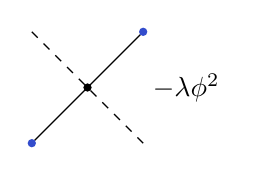
\begin{tikzpicture}[scale=0.707]
    \draw (0, 0) node [circ, mblue] {} -- (2, 2) node [circ, mblue] {};
    \draw [dashed] (0, 2) -- (2, 0);
    \node [circ] at (1, 1) {};
    \node [right] at (2, 1) {$-\lambda \phi^2$};
  \end{tikzpicture}
\end{center}
For our accounting purposes, we will say the internal vertex contributes a factor of $-\lambda$, and each terminating blue vertex contributes a factor of $\phi$.

Since we have a ``constant'' term $\frac{m^2}{2} \phi^2$ as well, we need to add one more diagram to account for that. We allow a single edge of the form
\begin{center}
  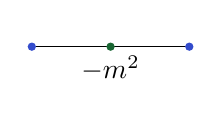
\begin{tikzpicture}
    \draw (0, 0) node [mblue, circ] {} -- (2, 0) node [mblue, circ] {} node [pos=0.5, below] {$-m^2$} node [pos=0.5, above] { };
    \node [circ, mgreen] at (1, 0) {};
  \end{tikzpicture}
\end{center}
With these ingredients, we can compute the effective potential as follows:
\[\everymath{\displaystyle}\arraycolsep=0.3em\def\arraystretch{2.2}
  \begin{array}{ccccccccccc}
    \displaystyle -S_{\mathrm{eff}}(\phi) &\sim&
  \begin{tikzpicture}[eqpic]
    \node [circ, mblue] at (0, 0) {};
    \node [circ, mblue] at (0, -2) {};
    \draw (0, 0) -- (0, -2);
  \end{tikzpicture}
  &+&
  \begin{tikzpicture}[eqpic]
    \node [circ, mblue] at (0, 0) {};
    \node [circ, mblue] at (0, -2) {};
    \draw (0, 0) -- (0, -2);

    \node [circ] at (0, -1) {};

    \draw [dashed] (0.4, -1) ellipse (0.4 and 0.25);
  \end{tikzpicture}
  &+&
  \begin{tikzpicture}[eqpic]
    \draw (0, 0) node [circ, mblue] {} -- +(0, -1) node [circ] {} -- +(0, -2) node [circ, mblue] {};
    \draw (0.8, 0) node [circ, mblue] {} -- +(0, -1) node [circ] {} -- +(0, -2) node [circ, mblue] {};
    \draw [dashed] (0.4, -1) ellipse (0.4 and 0.25);
  \end{tikzpicture}
  &+&
  \begin{tikzpicture}[eqpic]
    \draw (0, 0) node [circ, mblue] {} -- +(0, -1) node [circ] {} -- +(0, -2) node [circ, mblue] {};
    \draw (0.8, 0) node [circ, mblue] {} -- +(0, -1) node [circ] {} -- +(0, -2) node [circ, mblue] {};
    \draw (0.4, 0.25) node [circ, mblue] {} -- +(0, -1) node [circ] {} -- +(0, -2) node [circ, mblue] {};
    \draw [dashed] (0.4, -1) ellipse (0.4 and 0.25);
  \end{tikzpicture}
  &+&
  \cdots\\
  && \frac{-m^2}{2}\phi^2 &+& \frac{-\lambda}{4 M^2} \phi^2 &+& \frac{\lambda^2 \phi^4}{16 M^4} &+& \frac{- \lambda^3 \phi^6}{48 M^6} &+& \cdots
\end{array}
\]
These are just the terms we've previously found. There are, again, a few things to note
\begin{itemize}
  \item The diagram expansion is pretty straightforward in this case, because we started with a rather simple interacting theory. More complicated examples will have diagram expansions that are actually interesting.
  \item We only sum over connected diagrams, as $S_{\mathrm{eff}}$ is the logarithm of the integral.
  \item We see that the new/shifted couplings in $S_{\mathrm{eff}} (\phi)$ are generated by \emph{loops} of $\chi$ fields.
\end{itemize}

\begin{eg}
  We can use the effective potential to compute $\bar \phi^2 \ket$:
  \[\everymath{\displaystyle}\arraycolsep=0.3em\def\arraystretch{2.2}
    \begin{array}{ccccccc}
      \displaystyle \bra \phi^2 \ket &\sim&
      \begin{tikzpicture}[eqpic]
        \node [circ] at (0, 0) {};
        \node [circ] at (0, -2) {};
        \draw (0, 0) -- (0, -2);
      \end{tikzpicture}
      &+&
      \begin{tikzpicture}[eqpic]
        \node [circ] at (0, 0) {};
        \node [circ] at (0, -2) {};
        \draw (0, 0) -- (0, -2);

        \node [circ] at (0, -1) {};

        \draw (0.4, -1) ellipse (0.4 and 0.25);
      \end{tikzpicture}
      &+&
      \cdots\\
      && \frac{1}{m_{\mathrm{eff}}^2} &+& \frac{-\lambda}{2m^6_{\mathrm{eff}}} &+& \cdots
    \end{array}
  \]
  We can see that this agrees with our earlier calculation correct to order $\lambda^2$.
\end{eg}

At this moment, this is not incredibly impressive, since it takes a lot of work to compute $S_{\mathrm{eff}}(\phi)$. But the computation of $S_{\mathrm{eff}}(\phi)$ can be reused to compute any correlation involving $\phi$. So if we do many computations with $\phi$, then we we can save time.

But the point is not that this saves work. The point is that this is what we do when we do physics. We \emph{have} to do this if we don't really know anything about $\chi$, but we can try to figure out $S_{\mathrm{eff}}(\phi^2)$ by working with experiments.

\section{QFT in one dimension (ie. QM)}
In $d = 1$, there are two possible connected, compact manifolds $M$ --- we can have $M = S^1$ or $M = I = [0, 1]$. % picture

When $M = I$, our universe has boundaries, which will need us to specify boundary conditions on the field in the path integral. This is a new feature.

We begin by considering the second case, and we'll let $t \in [0, 1]$ be a worldline coordinate. We consider a field
\[
  x: I \to N
\]
for some Riemannian manifold $(N, g)$, which we call the \term{target manifold}. If $U\subseteq N$ has coordinates $x^a$ with $a = 1, \cdots, n = \dim (N)$, then we usually write $x^a(t)$ for the coordinates of $x(t)$.

The standard choice of action is
\[
  S[x] = \int_I \left(\frac{1}{2} g_{ab}(x) \dot{x}^a \dot{x}^b + V(x)\right)\;\d t,
\]
where
\[
  \dot{x}^a = \frac{\d x^a}{\d t}.
\]
In this case, the theory is called a \term{non-linear $\sigma$-model}. It is called $\sigma$-model because when people first wrote this theory down, they used $\sigma$ for the name of the field, and the name stuck. This is non-linear because the term $g_{ab}(x) \dot{x}^a \dot{x}^b$ can be very complicated when the metric $g_{ab}$ if it is not flat. Note that $+V(x)$ is the correct sign for a Euclidean worldline.

The extrema of $S[x]$ (for fixed end points) obey the equation
\[
  \frac{\d^2 \dot{x}^a}{\d t^2} + \Gamma^a\!_{bc} \dot{x}^b \dot{x}^c = g^{ab} \frac{\partial V}{\partial x^a}.
\]
Here the right-hand side describes some non-gravitational force.

How is this related to quantum mechanics? The standard way to do quantum mechanics on $N$ is to pick a Hilbert space $\mathcal{H}$, which is typically $\mathcal{H} = L^2(N, \d \mu)$, the space of square-integrable functions on $N$. Also, to describe dynamics, we pick a Hamiltonian operator $H: \mathcal{H} \to \mathcal{H}$, with the usual choice being
\[
  H = \frac{1}{2} \Delta + V,
\]
where
\[
  \Delta = \frac{1}{\sqrt{g}} \partial_a(\sqrt{g} g^{ab} \partial_b).
\]
In this case, the amplitude for a particle to travel from $x \in N$ to $y \in N$ in Euclidean time $T$ is
\[
  K_T(y, x) = \brak{y} e^{-HT}\bket{x}.
\]
This is in the Heisenberg picture. In the Schr\"odinger picture, it is
\[
  \braket{y, T}{x, 0}.
\]
Here $K_T(y, x)$ is defined to be the unique solution of
\[
  \frac{\partial}{\partial t} K_t(y, x) + H K_t(y, x) = 0
\]
such that
\[
  \lim_{t \to 0} K_t(y, x) = \delta^a (y - x).
\]
Here we view $K_t(y, x)$ as a function of $x$, so that $H$ can act on it.

(Note that if we replace $t$ with $it$, then we have
\[
  i \frac{\partial K_t}{\partial t} (y, x) = H K_t(y, x).
\]
which is the Schr\"odinger equation)

This $K_t(y, x)$ is often called the \term{heat kernel} on $(N, g, V)$.
\begin{eg}
  Consider $(N, g, V) = (\R^n, \delta, 0)$, then we have
  \[
    K_t(y, x) = \frac{1}{(2\pi t)^{n/2}} \exp\left(-\frac{|x - y|^2}{2t}\right).
  \]
  More generally, for an arbitrary $(N, g, V) = (N, g, 0)$, then it is very hard to write down the closed form expression for $K$. However, we can find the asymptotic form
  \[
    \lim_{t \to 0} K_t(y, x) \sim \frac{a(x)}{(2\pi t)^{n/2}} \exp\left(- \frac{d(y, x)^2}{2t}\right),
  \]
  where $d(x, y)$ is the geodesic distance between $x$ and $y$, and $a(x)$ is some invariant of our manifold built from (integrals of) polynomials of the Riemann curvature.
\end{eg}
We can also view $K_t(x, y)$ as a path integral. Let
\[
  \Delta t = \frac{t}{N}
\]
for some large $N \in \N$. Then we have
\[
  K_t(y, x) = \brak{y} e^{-TH} \bket{x} = \brak{y} e^{-\Delta t H} e^{-\Delta tH} \cdots e^{-\Delta t H} \bket{x}.
\]
We can now insert the identity operator between the different operators, and this becomes
\begin{align*}
  K_{t}(y, x) &= \int \prod_{i = 0}^{N - 1} \d^n x_i \brak{y}e^{-\Delta t H}\bket{x_{N - 1}} \brak{x_{N - 1}}e^{-\Delta t H}\bket{x_{N - 2}} \cdots \brak{x_1} e^{-\Delta H t} \bket{x}\\
  &= \int \prod_{i = 1}^{N - 1} \d^n x_i K_{\Delta t} (x_i, x_{i - 1}),
\end{align*}
where we conveniently set $x_0 = x$ and $x_N = y$.

This follows from the concatenation property of the heat kernel, ie.
\[
  K_{t_1 + t_2}(y, x) = \int \d^n z K_{t_2}(y, z) K_{t_1}(z, x).
\]
For flat space, this is just reduces to the formula for convolution of Gaussians.

The purpose of introducing these $\Delta t$ is that we can now use the asymptotic form of $K_t(y, t)$. Consequently, we can say
\[
  \brak{y_1} e^{-HT} \bket{y_0} = \lim_{N \to \infty} \left(\frac{1}{2\pi \Delta t}\right)^{nN/2} \int \prod_{i = 1}^{N - 1} \d^n x_i\; a(x_i) \exp\left(- \frac{\Delta t}{2}\left(\frac{d(x_{i + 1}, x_i)}{\Delta t}\right)^2\right).
\]
This looks more-or-less like a path integral! \emph{IF} we declare the path integral measure
\[
  \D x \overset{?}{\equiv} \lim_{N \to \infty} \left(\frac{1}{2\pi \Delta t}\right)^{nN/2} \prod_{i = 1}^{N - 1} \d^n x_i\; a(x_i),
\]
and \emph{IF} our map $x(t)$ is at least once-continuously differentiable, then we can write
\[
  \lim_{N \to \infty} \prod_{i = 1}^{N - 1} \exp\left(-\frac{\Delta t}{2} \left(\frac{d(x_{i + 1}, x_i)}{\Delta t}\right)^2 \right) = \exp\left(-\frac{1}{2} \int \d t\; g_{ab} \dot{x}^a \dot{x}^b\right) = \exp(-S[x]).
\]
Note that this is all done for $V = 0$, which was assumed for the asymptotic series of the heat kernel to hold.

Under these assumptions, we have
\[
  \brak{y_1} e^{-HT} \bket{y_0} = \int_{\mathcal{C}_T[y_1, y_0]} \D x\; \exp\left(-\int \frac{1}{2} g_{ab} \dot{x}^a \dot{x}^b\;\d t\right),
\]
where $\mathcal{C}_T[y_1, y_0]$ is the space of ``all'' continuous maps $I \to N$ such that $x(0) = y_0$ and $x(1) = y_1$.

Note that $\bket{y_0} \in \mathcal{H}$ and $\brak{y_1} \in \mathcal{H}^*$ used to evaluate our propagator here arise as boundary conditions on the map $x$.

The fact that these states in $\mathcal{H}$ are associated with these codimension-1 subspaces of the manifold is something we have seen before. When we did quantum field theory, almost everything we did was for equal times. Even in the Heisenberg picture, the commutation relations are given for equal times, not in general. This is since we were not working with the entire Minkowski space, but only ``equal time'' codimension-1 slices.

\subsubsection*{The partition function}

We also have the object $\Tr_\mathcal{H}(e^{-HT})$, which is what we usually call the partition function in statistical mechanics, and it is given by
\[
  \Tr_H(e^{-HT}) = \int \d^n y\; \brak{y}e^{-HT} \bket{y}.
\]
Using our path integral formulation, we can write this as
\[
  \Tr_\mathcal{H} (e^{-HT}) = \int \d^n y \int_{C_I[y, y]} \D x\; e^{-S} = \int_{\mathcal{C}_{S^1}} \D x\; e^{-S},
\]
where we integrate over all circles. This is the partition function $\mathcal{Z}(S^1, (N, g, V))$ of our theory.

So in the presence of boundaries, we can obtain matrix elements, and on a closed compact manifold, we get the partition function.

We can also do correlation functions. The simplest choice of correlation functions is a \emph{local operator}.
\begin{defi}[Local operator]\index{local operator}
  A \emph{local operator} $\mathcal{O}(t)$ is one which depends on the values of the fields and finitely many derivatives just at one point $t \in M$.
\end{defi}
The simplest type come from functions on $N$, ie. if $\mathcal{O}: N \to \R$, then by pullback we get an operator $\mathcal{O}(x^a(t))$.

Normally, in quantum mechanics, we want to compute
\[
  \brak{y_1} \hat{\mathcal{O}}(t) \bket{y_0} = \brak{y_1} e^{-H(T - t)} \hat{\mathcal{O}} e^{-Ht} \bket{y_0},
\]
where $\hat{\mathcal{O}} = \mathcal{O}(\hat{x})$.

But, inserting a complete set of states, this is equal to
\[
  \int \d^n x\; \brak{y_1} e^{-H(T - t)}\bket{x} \brak{x}\hat{\mathcal{O}} e^{-Ht} \bket{y} = \int \d^n x\; \mathcal{O}(x) \brak{y_1} e^{-H(T - t)} \bket{x} \brak{x} e^{-Ht} \bket{y},
\]
where we use the fact that $\hat{\mathcal{O}}(x) \bket{x}  = \mathcal{O}(x) \bket{x}$. In other words, we find
\[
  \brak{y_1} \hat{\mathcal{O}}(t) \bket{y_0} = \int \d^n x\; \mathcal{O}(x(t)) \int_{\mathcal{C}_{[T, t]} [y_1, x_t]} e^{-S[x]} \int_{\mathcal{C}_{[t, 0]}[x_t, y_0]} \D x\; e^{-S[x]}.
\]
But this is just the same as
\[
  \int_{\mathcal{C}_{[T, 0]}[y_1, y_0]} \D x\; \mathcal{O}(x(t)) e^{-S[x]}.
\]
What we have seen is that as long as we are willing to make the (rather unsubstantiated) assumptions that we can do path integrals, then we have managed to interpret a lot of things we've seen in quantum mechanics in terms of path integrals.


\printindex
\end{document}
